\documentclass[border=10pt]{standalone}
\usepackage{pgfplots}
\usepgfplotslibrary{fillbetween}
\pgfplotsset{compat=1.18}
\begin{document}
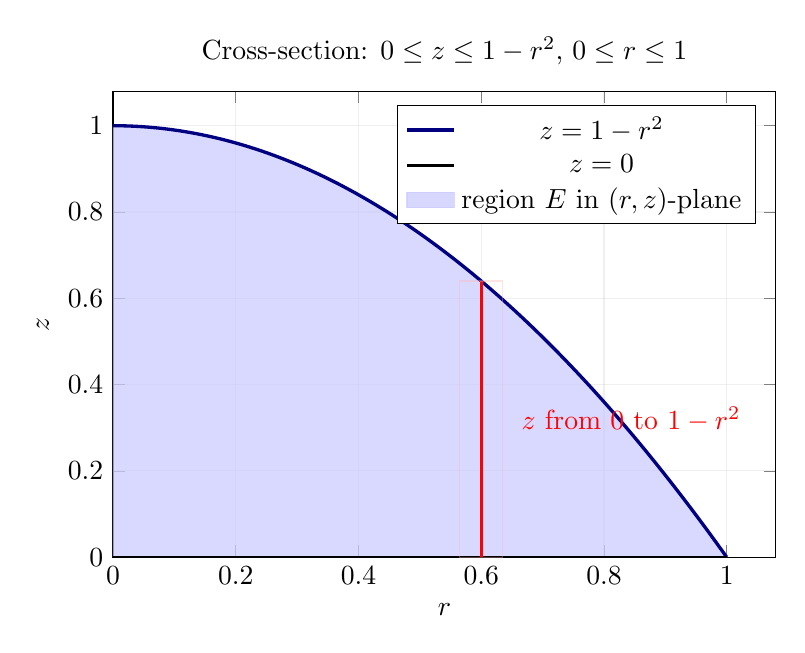
\begin{tikzpicture}
\begin{axis}[
    width=10cm, height=7.5cm,
    xlabel={$r$}, ylabel={$z$},
    xmin=0, xmax=1.08, ymin=0, ymax=1.08,
    domain=0:1, samples=120,
    grid=both, grid style={opacity=0.25},
    title={Cross-section: $0\le z\le 1-r^2$, $0\le r\le 1$},
    legend pos=north east,
]
\addplot[name path=A, blue!50!black, very thick] {1-x^2};
\addlegendentry{$z=1-r^2$}
\addplot[name path=B, black, thick] {0};
\addlegendentry{$z=0$}
\addplot[blue!20, opacity=0.75] fill between[of=A and B];
\addlegendentry{region $E$ in $(r,z)$-plane}
\addplot[red, very thick, forget plot] coordinates {(0.6,0) (0.6,0.64)};
\addplot[red!30, opacity=0.35, forget plot] coordinates {(0.565,0) (0.635,0) (0.635,0.64) (0.565,0.64)} \closedcycle;
\node[red, anchor=west] at (axis cs:0.65,0.32) {$z$ from $0$ to $1-r^2$};
\end{axis}
\end{tikzpicture}
\end{document}
